\section{Introduction}
%Commonsense knowledge is an important ingredient in machine comprehension and
%inference. 
Artificial Intelligent systems can benefit from incorporating commonsense knowledge as background, 
such as \textit{ice is cold} (\textsc{HasProperty}), 
\textit{chewing is a sub-event of eating} (\textsc{HasSubevent}), 
\textit{chair and table are typically found near each other} (\lnear), etc. 
This kind of commonsense facts have been utilized in many downstream tasks, such as textual entailment~\cite{dagan2009recognizing,bowman2015large} and visual recognition tasks~\cite{zhu2014reasoning}.
The commonsense knowledge is often represented as relation triples in commonsense knowledge bases, 
such as \textit{ConceptNet} by MIT \cite{speer2012representing}, one of the largest commonsense
knowledge graph available today.
However, this kind of commonsense knowledge bases are usually manually curated or crowd-sourced by community efforts and thus do not scale well.
%For example, ConceptNet contains only 49 \lnear~relation triples. 
%%Many commonly co-located objects such as (house, garden) and 
%%(fork, knife) are not included in this knowledge base. 
%Another problem is that such commonsense knowledge bases are typically contributed by just a very limited number of people due to the cost of manual labor. 
%Thus no meaningful statistical scores can be
%associated with the triples, making rank-based 
%computation difficult. 
%For instance, although ConceptNet gives a confidence
%score (from 0 to infinity) to each triple, most of the triples have the default
%score of 1, simply because the human contributor did not or could not 
%provide a score. 
%If such commonsense knowledge is harnessed automatically
%from open-domain text corpora, both of the above problems can be 
%effectively addressed. 
%Open information extraction not only provides the much needed scale,
%but also valuable statistics that can turn into confidence scores.

This paper aims at automatically extracting the commonsense \lnear\ relation between
physical objects from textual corpora, which is defined as two objects typically found near each other in real life.
%\footnote{Because some physical objects can be a location itself, this
%relation may include some instances of the \textsc{atLocation} relation,
%e.g., {\em room} and {\em door}.}
We focus on \lnear\ relation for these reasons:  
	(i) \lnear\ facts are helpful prior knowledge for object detection in complex image scenes; \figref{fig:dim} illustrates two motivating examples;
	%(The guess can be based on commonsense knowledge learned from room settings scene description in articles and texts.)
	%Such prior knowledge helps with the object detection accuracy; 
	(ii) such commonsense knowledge can potentially benefit general reasoning in reading comprehension,
	question answering as well as many other AI tasks;
	(iii) existing knowledge bases have very few facts for	this relation (\textit{ConceptNet 5} has only 49 triples of \lnear). 
\begin{figure}[bh]
	\centering
	\begin{subfigure}{.45\textwidth}
		\centering
		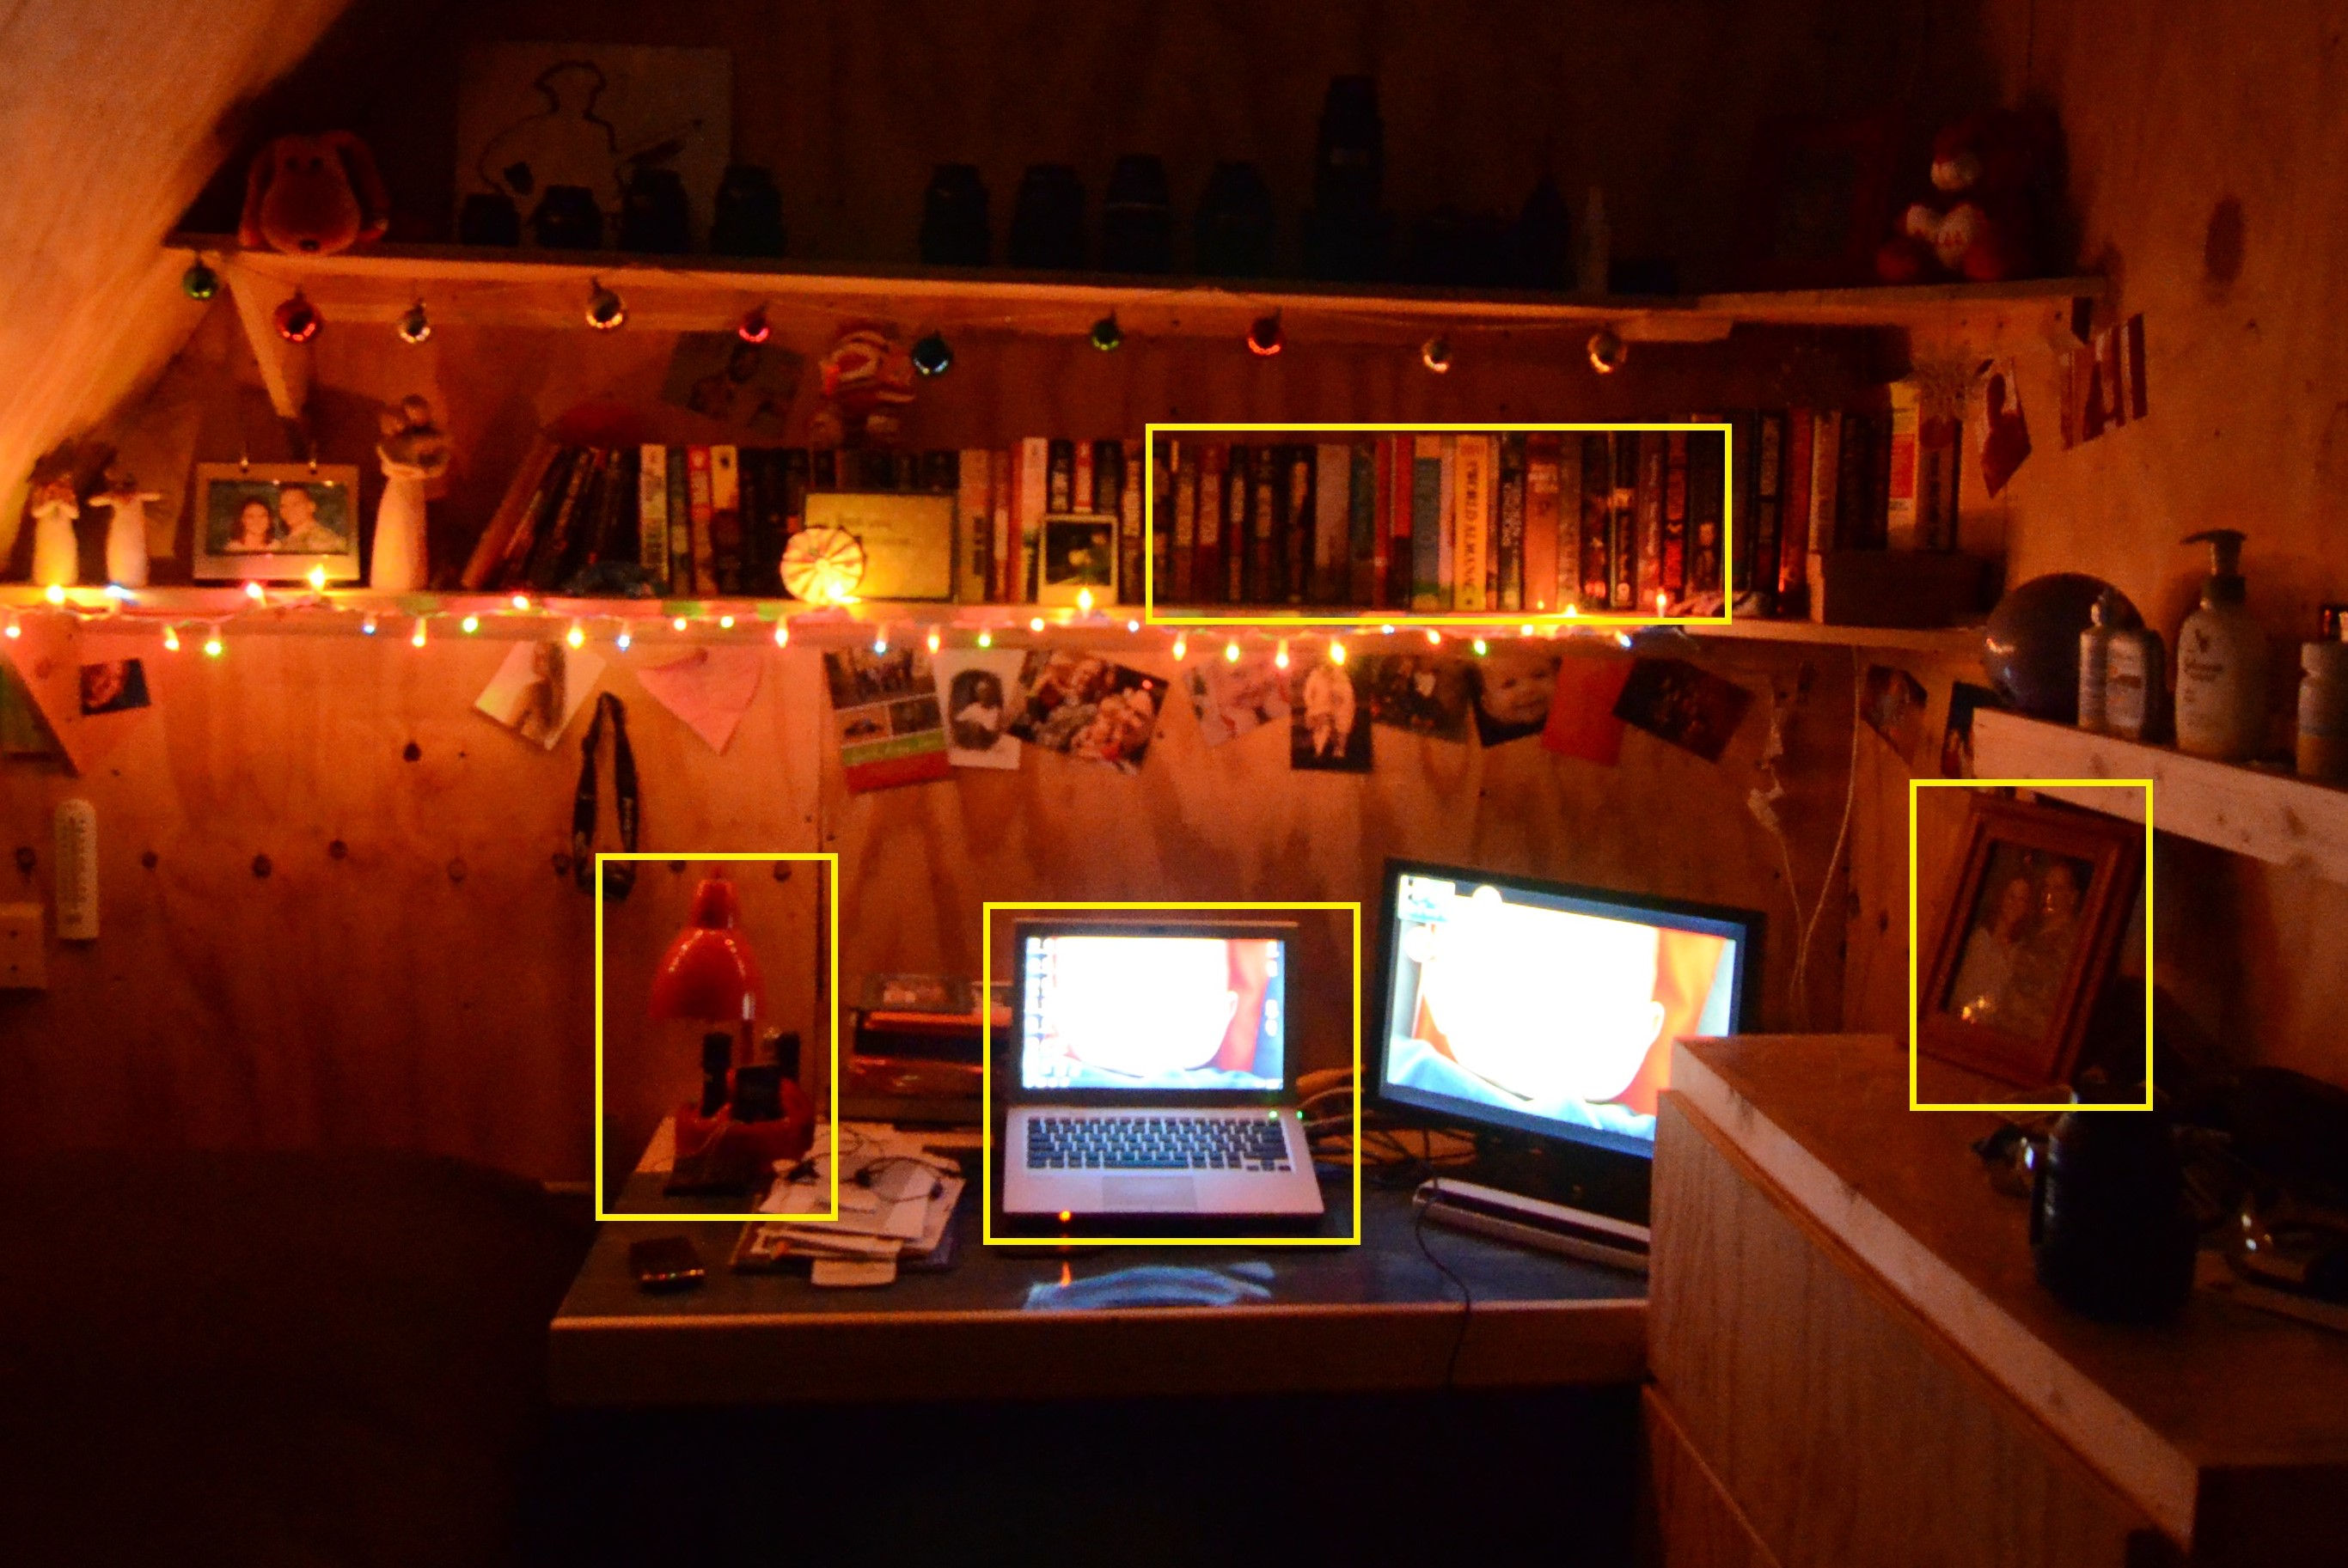
\includegraphics[width=0.95\columnwidth]{dim-room.jpg}
	\end{subfigure}
	\begin{subfigure}{.45\textwidth}
		\centering
		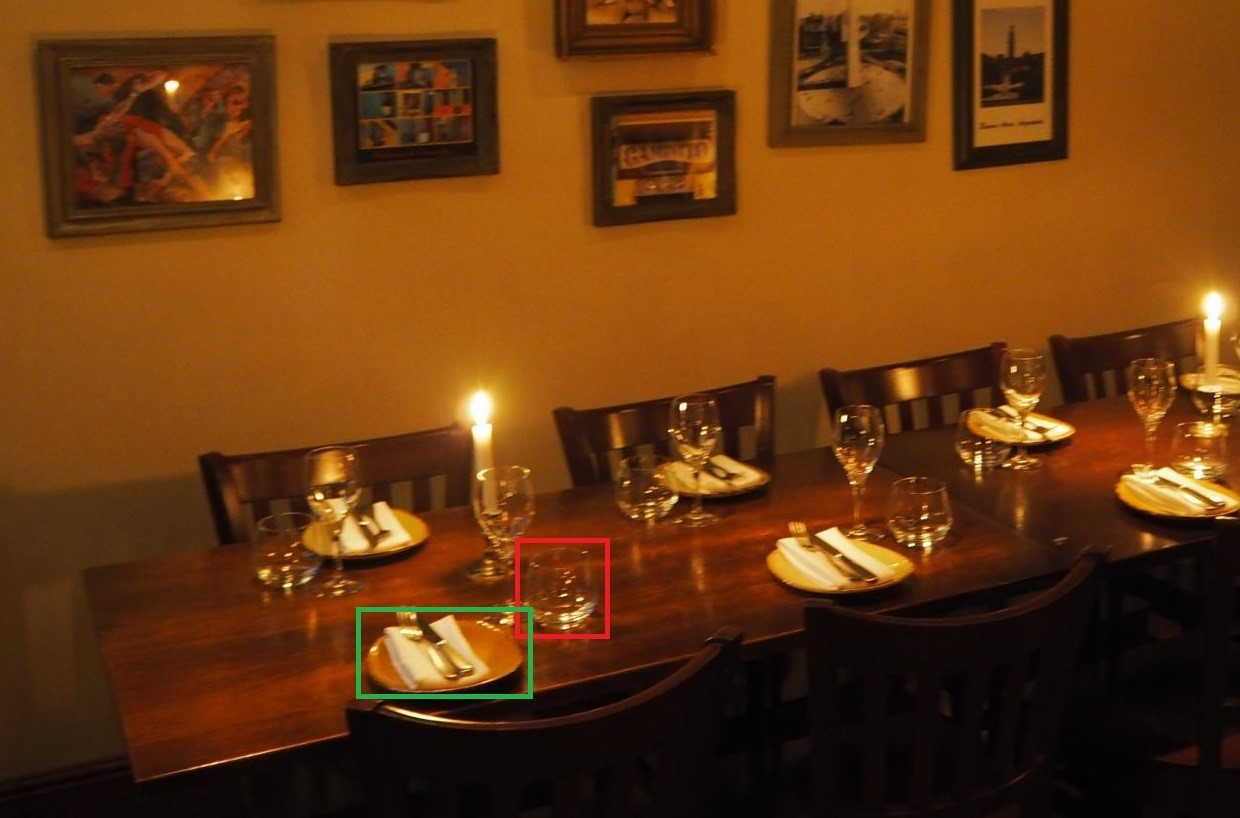
\includegraphics[width=0.95\columnwidth]{dim-table.jpg}
	\end{subfigure}
	\caption{\lnear~relation facts assist the detection of vague objects: in a dimly lit room with settings shown in the \textit{left sub-figure}, if a bright laptop is present on a table, one may guess that a lamp, a photo frame or books maybe nearby. Similarly in the \textit{right sub-figure}, if a set of knife, fork and plate is on the table, one may believe there could be a glass beside based on the commonsense, 
		even though these objects are hardly visible due to low light.}
	\label{fig:dim}
\end{figure}
%
%\begin{enumerate}
%\item \lnear relation is useful for object detection in complex image 
%scenes. For example, in a dimly lit room with a dining table and some chairs.
%One may guess that plates and other kitchenware maybe present on the table.
%Such prior knowledge helps with the object detection accuracy. \KZ{give a 
%real image here which is hard to detect by state-of-the-art algo but 
%obeys commonsense.}
%
%%\item \lnear relation can also be useful for automated conversation systems
%%where meaningful context maybe added to the conversation. \KZ{Example?}
%
%\item \lnear relation can benefit general reasoning in reading comprehension,
%question answering and many other AI tasks.
%
%\item Existing knowledge bases such as Concept Net has very limited facts for
%this relation.
%\end{enumerate}

%Automatic extraction of relations from open text has a short but rich history. 
%Attempts have been made to extract isA, causal, correlation, and 
%also open domain relations (e.g., ReVerb, Yago).
%%\KZ{cite and Say more about KBC}. 
%\lnear~relation is unique and poses significant challenges
%for the following reasons:
%
%i) It involves physical (often visible) objects whereas other 
%popular relations involve general concepts or just natural language terms. 
%
%ii) The distribution of \lnear~ relation is not even across domains: 
%it is more prevalent in literary work such as stories 
%and dramas which come with descriptive scenes rather
%than in news, science \& technology related articles or online user 
%generated content. 
%%Our preliminary investigation shows that XXX\% of the sentences 
%%in New York Times and YYY\% of the sentences
%%in Wikipedia contains a \lnear~ relation, 
%%while that percentage for novels and stories in Gutenberg corpus is ZZZ\%. 
%
%iii) Sentences in literature are often complex and nuanced, 
%which makes extraction particularly challenging. Consider the objects
%``bed'' and ``star'' in the following
%sentence: ``{\em Until at last all the promenaders had gone home to bed, 
%and I was alone with the star.}'' Bed is not near the star
%because it's at another location.
%
%iv) Labeling such sentence is a non-trivial task, 
%and obtaining a large training set is difficult and expensive.
%
%\BL{add more related work about KBC here, mainly about Xiang Li (TTIC) and Stating the Obvious; to stress that why we are using raw text}

%Since raw text of novels tend to contain many 
%descriptions of  scene in real life, 
%we argue that it is feasible to obtain unseen 
%{\lnear} relations from raw novel text. 
%\vspace{-10pt}
We propose two novel tasks in extracting \lnear\ relation from textual corpora.
One is a binary relation classification problem which judges whether or not
a sentence is describing two objects physically close by.
The other task is to produce a ranked list of \lnear\
facts with the given classified results of 
large number of sentences. 
We believe both two tasks can help the community further automatically complete and populate existing commonsense knowledge bases.
%Notice that two objects that are {\em co-located} in a couple of sentences
%may not mean they have the \lnear\ relation as commonsense.

Additionally, we also create two benchmark datasets for evaluating \lnear~relation extraction systems on the two tasks: one is 5,000 sentences 
each describing a scene of two physical objects and with a label indicating if the two objects are co-located in the scene; 
the other consists of 500 pairs of objects with human-annotated scores indicating confidences that a certain pair of objects are commonly located near in the real life. 

%is to build a framework to automatically extract 
%large amount of unseen object pairs with \lnear relations 
%from literary text corpora.
%that 
%are not already included in ConceptNet. \KZ{Need to back up this claim in eval}
%Considering the fact that not all sentences mentioning two physical objects 
%indicate that the two objects are nearby each other, 
%our proposed approach is to first construct a sentence-level relation classification model 
%to identify \lnear~ relation and then score each candidate object pair with the model 
%and the sentences containing it.
%Thus, the core problem is to judge whether a given sentence 
%containing two objects is describing a \lnear~ relation between the two objects or not. 
%

%More formally, given a sentence $s$ mentioning a pair of physical objects 
%\textless$e_1,e_2$\textgreater, 
%the problem is to determine whether $e_1$ and $e_2$ are located near each other in a physical scene 
%described in the sentence $s$. 
%
%\begin{table}[th!]
%	\centering
%	\caption{Examples for sentence-level \lnear Classification; The  \textless$e_1,e_2$\textgreater in both instances is \textless dog,cat\textgreater. Since the the first sentence is describing a physical scene about the dog and the cat, 
%		while the dog and the cat in the second sentence do not have to be located near since it is just talking about a general comparison.}
%	\label{tbl:lnc}
%	\begin{tabular}{|c|c|}
%		\hline
%		$s$    &  T/F\\ \hline
%	My dog is older than her cat.	 &  T\\ \hline
%	The King put his dog and cat on the table.     & F  \\ \hline
%	\end{tabular}
%
%\end{table}
%
%\KZ{Can use the two examples earlier. 
%For example, suppose $s_1$ = ``The King put his dog and cat on the table.'', 
%$s_2$ = ``My dog is older than her cat.'', 
%$e_1$ is ``dog" and $e_2$ is ``cat''. 
%Then the answer of $s_1$ is \textit{True} and of  $s_2$ is \textit{False} , 
%since the $s_1$ is describing a physical scene about the dog and the cat, 
%while the dog and the cat in $s_2$ do not have to be located near since it is just talking about a general comparison.
%}

%\BL{Add related work here about the relation classification , and their shortcoming (too many parameters) }

We propose several methods to solve the tasks including feature-based and LSTM-based neural architecture. 
The proposed neural architecture compares favorably with the current state-of-the-art method for general-purpose relation classification problem.
From our relatively smaller proposed datasets, we extract in total 2,067 new \lnear~triples that are not in \textit{ConceptNet}.


